%%%%%%%%%%%%%%%%%%%%%%%%%%%%%%%%%%%%%%%%%%%%%%%%%%%%%%%%%%%%%%%%%%%%%%%%%%%%%%%%
% Overview
%%%%%%%%%%%%%%%%%%%%%%%%%%%%%%%%%%%%%%%%%%%%%%%%%%%%%%%%%%%%%%%%%%%%%%%%%%%%%%%%
% Briefly tell the audience what you are going to cover.
\subsection{Overview}
\begin{frame}[label=overview]{Overview}
    \begin{itemize}
        \note{In this presentation, I will discuss the works and results of my
            \thesis{} project, which was conducted during the year of 2012 under
            the supervision of \supervisorName{}, and with assistance from PhD
            student \getPerson{Frechtling}.}

        \item<1-> Analysis and benchmarking of an anomaly detection algorithm.
        \note[item]<1>{I will provide an overview of my analysis and
            benchmarking of an existing anomaly detection algorithm. This
            algorithm:}
        \begin{itemize}
            \item Uses commute time as a distance metric.
            \note[item]{Uses commute time as a distance metric. Commute time
                effectively captures both the distance between nodes, as well as
                the data density around these nodes.}

            \item Uses eigenspace embedding.
            \note[item]{The use of Eigenspace embedding alleviates the $O(n^3)$
                computational complexity of the commute time calculations.}
            \note[item]{The graph components are sampled in order to reduce the
                graph size, and then Eigenspace approximation is applied to
                approximate the commute time on the sampled graph.}
        \end{itemize}

        \item<2-> Exploration of the use of reconfigurable computing to solve
            computing problems.
        \note[item]<2>{Reconfigurable computing is the application of
            \glspl{FPGA} to solve computing problems.}
        \note[item]<2>{\glspl{FPGA} are devices that combine the advantages of
            hardware implementations (speed) with the flexibility of software
            implementations (configurability).}

        \item<3-> Discuss an architecture design for using hardware to
            accelerate algorithms that involve repeated pairwise computations.
        \note[item]<3>{I will also discuss an architecture which I have designed
            for the acceleration of a class of algorithms using reconfigurable
            hardware.}
    \end{itemize}
\end{frame}

\begin{frame}[label=algorithm-performance]{Algorithm Performance}
    \begin{columns}[c]
        \column{0.5\textwidth}
        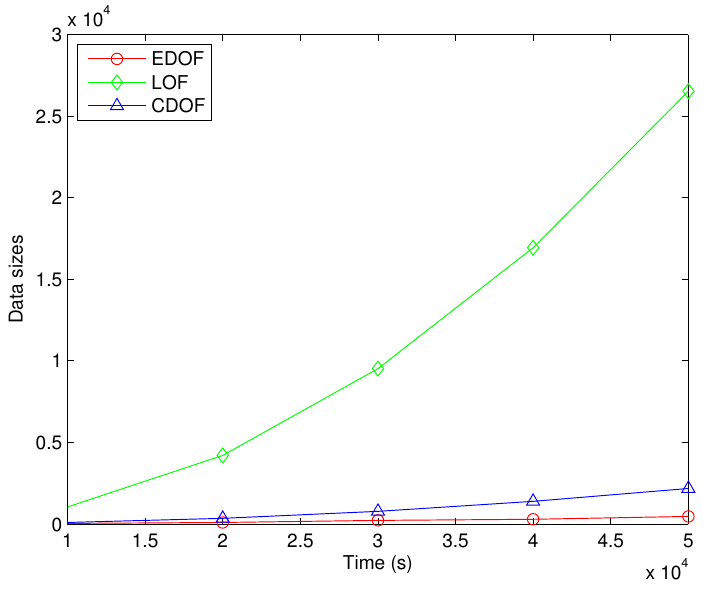
\includegraphics[width=\textwidth]{algorithm/run-time}

        \column{0.5\textwidth}
        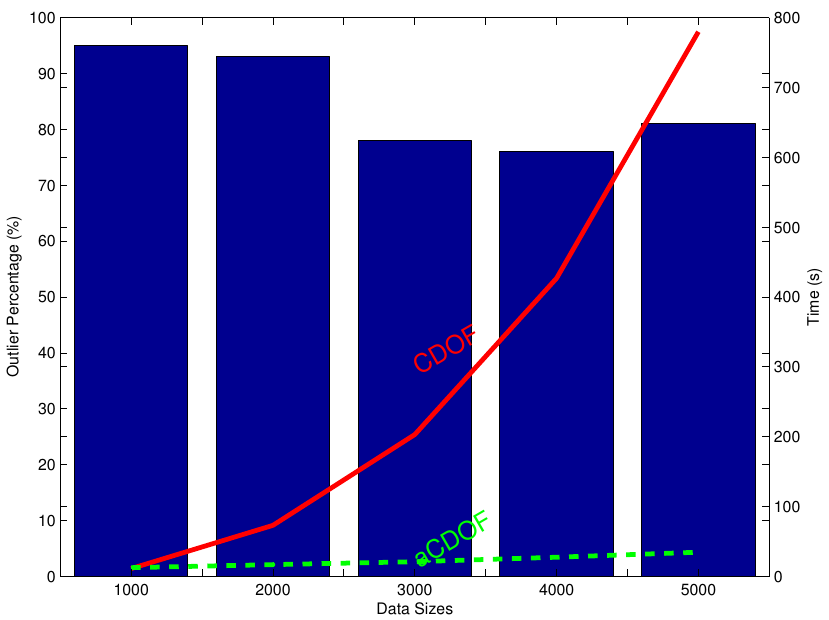
\includegraphics[width=\textwidth]{algorithm/accuracy}
    \end{columns}

    \note{
        These graphs show the measured performance of the chosen algorithm.

        \begin{itemize}
            \item Run time (using \emph{approximated} commute time) is
                proportional to $O(n \log n)$, compared to:
            \begin{itemize}
                \item $O(n)$ using Euclidean distance.
                \item $O(n^2)$ using \gls{LOF}.
            \end{itemize}

            \item Anomaly detection using \emph{approximated} commute time
                preserves a high percentage (84.6\% on average) of top anomalies
                discovered without using approximations.
            \end{itemize}}
\end{frame}

%%%%%%%%%%%%%%%%%%%%%%%%%%%%%%%%%%%%%%%%%%%%%%%%%%%%%%%%%%%%%%%%%%%%%%%%%%%%%%%%
% Motivation
%%%%%%%%%%%%%%%%%%%%%%%%%%%%%%%%%%%%%%%%%%%%%%%%%%%%%%%%%%%%%%%%%%%%%%%%%%%%%%%%
% Briefly tell the audience why you are doing your research. Sell your audience
% on why your topic is important and of interest to them.
\subsection{Motivation}
\begin{frame}[label=motivation]{Motivation}
    \begin{itemize}
        \item The amount of data being collected and stored is continually
            increasing.
        \item Anomaly detection is an important technique which can be applied
            to a wide range of applications.
    \end{itemize}
\end{frame}

\begin{frame}[label=applications]{Applications}
    \note{Anomaly detection is an interesting problem with a wide range of
        applications, including:}
    \begin{itemize}
        \item Stock market analysis
        \note[item]{Stock market analysis}

        \item Network intrusion detection
        \note[item]{Network intrusion detection}

        \item Image comparison
        \note[item]{Image comparison}

        \item Fraud detection
        \note[item]{Fraud detection}

        \item Data cleaning
        \note[item]{Data cleaning}

        \item Detecting employers with poor injury histories
        \note[item]{Detecting employers with poor injury histories}
    \end{itemize}
\end{frame}

%%%%%%%%%%%%%%%%%%%%%%%%%%%%%%%%%%%%%%%%%%%%%%%%%%%%%%%%%%%%%%%%%%%%%%%%%%%%%%%%
% Aims
%%%%%%%%%%%%%%%%%%%%%%%%%%%%%%%%%%%%%%%%%%%%%%%%%%%%%%%%%%%%%%%%%%%%%%%%%%%%%%%%
% This section should be short and memorable.
\subsection{Aims}
\begin{frame}[label=aims]{Aims}\relax
    {\huge To \emph{investigate} the \emph{performance benefits} that can be
        obtained by \emph{applying} \emph{reconfigurable computing design
        principles} to an \textbf{anomaly detection algorithm} using commute
        time and eigenspace sampling.}

    \note{The aim of this \thesis{} was to \emph{investigate} the
        \textbf{performance benefits} that can be obtained by \emph{applying}
        \textbf{reconfigurable computing design principles} to an
        \textbf{anomaly detection algorithm} using commute time and eigenspace
        sampling.}
\end{frame}

%%%%%%%%%%%%%%%%%%%%%%%%%%%%%%%%%%%%%%%%%%%%%%%%%%%%%%%%%%%%%%%%%%%%%%%%%%%%%%%%
% Contributions
%%%%%%%%%%%%%%%%%%%%%%%%%%%%%%%%%%%%%%%%%%%%%%%%%%%%%%%%%%%%%%%%%%%%%%%%%%%%%%%%
% What I contributed towards this research area.
\subsection{Contributions}
\begin{frame}[label=contributions]{Contributions}
    \begin{enumerate}
        \item Quantitative analysis and benchmarking of the properties of the
            chosen anomaly detection algorithm.
        \begin{itemize}
            \item Justify why we worked on that.
        \end{itemize}
        \item An architecture for accelerating a wide class of algorithms.
        \begin{itemize}
            \item Other examples of where this design could be applied.
        \end{itemize}
        \item Implementation
    \end{enumerate}
\end{frame}
